\section{Introduction}\label{sec:intro}

\IEEEPARstart{C}{ylinder} chess is ordinary chess played on a board whose a-file and h-file are joined
\cite{Pritchard}. A white pawn on h4 can capture on a5, a king on a1 can step to h2, and every file is like every
other: the board has no edges and no corners (Fig.~\ref{fig:cover}). In this paper we use combinatorial game
theory (CGT) to study king-and-pawn endgames on this board.

Under normal play, the player who cannot move loses. CGT gives each position of such a game a value, and the
value of a sum of independent games is the sum of their values \cite{ONAG,WinningWays,Siegel2013}. Chess is not
such a game: it can be drawn, and the kings can walk from one part of the board to another. Even so, Elkies
\cite{Elkies1996} showed that many pawn endgames split into local fights whose values are numbers, star,
infinitesimals such as up, and hot switches. Two conventions make this work:
\begin{itemize}
\item a side that gets a passed pawn wins, so a passed pawn is worth a large number $\pm\BIG$;
\item the kings stand in a mutual zugzwang, the \emph{tr\'ebuchet}, which counts as $0$.
\end{itemize}
Wu, Y\"u and Landry \cite{WuYuLandry2020} worked through these ideas position by position, and we follow
their format.

The cylinder changes this picture in three ways. There are no rook pawns, and a position can be shifted
sideways by any number of files without changing its value. A position with a pawn on every file, a
\emph{ring}, has no edge at which to cut it. And the corners that decide mates and fortresses on the ordinary
board are gone.

\begin{figure}[!t]
\centering
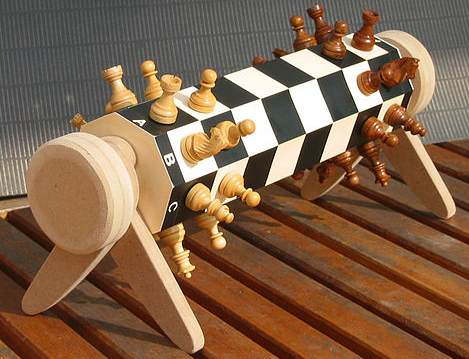
\includegraphics[width=0.6\columnwidth]{figures/CoverPic.png}
\caption{Cylindrical chessboard with all pieces on their starting squares; files a and h are adjacent.
Photograph by S.~Clair, Wikimedia Commons, CC BY-SA 3.0~\cite{CoverImage}.}
\label{fig:cover}
\end{figure}

The simplest nimber after $\star$ is $\nim{2}=\game{0,\star}{0,\star}$, a game in which either player may move
to $0$ or to $\star$. Elkies later built higher nimbers in pawn endgames on large boards by
adapting Dawson's pawn game \cite{Elkies2002,Dawson1935}, and Drummond-Cole gave positions of value $\nim{2}$
in generalized Domineering and in chess \cite{DrummondCole2005}. We ask whether $\nim{2}$ occurs in a
king-and-pawn endgame on a board with eight ranks, the \emph{$\nim{2}$ question}, and, where the model says
$\nim{2}$, whether real chess agrees.

This paper extends an unpublished 2025 study\bytheauthor~\cite{Bhattacharjee2025}, which built the basic
values on the cylinder by hand; here every position is checked by computer, the errors of that study are
corrected where they occur, and the analysis is carried on to the questions above. Because so much of the work
is computational, each theorem and headline number carries a label: \lab{P} proved, \lab{C2} checked by two
independent programs, \lab{C1} computed by one program, and \lab{Conj} a conjecture. Our contributions are as
follows.
\begin{itemize}
\item \emph{An exact model} (Sections~\ref{sec:rules} and~\ref{sec:sums}). The textbook passed-pawn test ignores
  en passant; we replace it, prove a cut lemma and a sum-safety theorem \lab{P}, and show that the earlier
  sum-safety test fails \lab{C2}.
\item \emph{Kings} (Section~\ref{sec:kings}). We give conditions (V1)--(V4) under which a frozen tr\'ebuchet
  gives the true chess result \lab{P}; on small boards the convention, with the textbook test, fails for 159 of
  500 components \lab{C1}.
\item \emph{Small values} (Sections~\ref{sec:atlas} and~\ref{sec:targets}). Every value that only the cylinder
  can make comes from a ring \lab{P}, and $1/8$, $\upsec\star$ and Tiny~1 occur in legal 10-man positions
  \lab{C2}.
\item \emph{The $\nim{2}$ question} (Section~\ref{sec:star2}). Under the new test no $\nim{2}$ exists with six
  pawns or fewer on boards of width at most four, but two exist with seven \lab{C2}.
\item \emph{Real chess} (Section~\ref{sec:real}). In the e.p.-aware pawn tree, the real-chess value of the
  textbook candidate is never $\nim{2}$, however draws are treated, and the $1/8$ hinges on one end position
  that a queen-promotion search leaves open \lab{C1}.
\item \emph{Tablebases} (Section~\ref{sec:tb}). On the cylinder king and rook win only 2.80\% of positions
  \lab{C2}.
\item \emph{Dawson's chess} (Section~\ref{sec:dawson}). The $3\times n$ cylinder is a first-player win if and
  only if the $3\times(n-3)$ strip has Grundy value $0$ \lab{P}.
\item \emph{Engines} (Section~\ref{sec:engines}). Stockfish is weakest on infinitesimals at low depth \lab{C1}.
\end{itemize}

Sections~\ref{sec:rules}--\ref{sec:basic} set up the rules and the basic values,
Sections~\ref{sec:kings}--\ref{sec:sums} add kings and sums, Sections~\ref{sec:atlas}--\ref{sec:real} search for
small values and test them against real chess, and Sections~\ref{sec:tb}--\ref{sec:engines} turn to tablebases,
Dawson's chess and engines. Section~\ref{sec:verify} explains how each result was checked, and
Section~\ref{sec:conclusion} lists open problems.
